\documentclass[11pt,a4paper]{article}
\usepackage[margin=2.3cm]{geometry}
\usepackage[T1]{fontenc}
\usepackage{amsmath,amssymb}
\usepackage{graphicx}
\usepackage{booktabs}
\usepackage{longtable}
\usepackage[round,authoryear]{natbib}
\usepackage[colorlinks=true,linkcolor=blue,citecolor=blue,urlcolor=blue]{hyperref}
\graphicspath{{figures_emissivity/}}
\newcommand{\flag}[1]{\textbf{\textcolor{red}{#1}}}
\usepackage{xcolor}

\title{Averaged ionizing emissivity of stellar photons and cosmic-ray
electrons,\\ counting all ionizations down the cascade\\
\large Hydrogen and helium branches}
\author{Response note --- \texttt{State of the art - Reionization/ionizing\_emissivity/}}
\date{10 September 2026}

\begin{document}
\maketitle

\begin{abstract}
\noindent
We compute, separately for hydrogen and for helium, three quantities as
functions of the energy of the primary particle: the number of ionizations
produced per primary particle counting every ionization down the cascade; the
differential ionizing emissivity per comoving volume; and the ionization rate
per target atom.  Two primary populations are treated, stellar
Lyman-continuum photons and cosmic-ray electrons, and two independent cascade
engines are run against each other throughout.  Every numerical input is
taken from a named paper; the only quantities computed rather than quoted are
two integrals (an IMF integral and a virial-theorem binding energy) that are
performed from scratch here and then checked against their published values.

The result is that cosmic-ray electrons deliver
$(3.8$--$7.5)\times10^{-5}$ of the hydrogen-ionizing emissivity of stellar
photons, and $(2.0$--$4.4)\times10^{-5}$ of the helium-ionizing emissivity,
essentially independently of redshift over $6\le z\le15$ and of the residual
ionized fraction over $10^{-4}\le x_e\le10^{-1}$.  Including the full range
spanned by the two published cosmic-ray injection prescriptions and their
efficiency uncertainties, the hydrogen share is
$5.8\times10^{-6}$--$4.7\times10^{-4}$ and the helium share
$3.1\times10^{-6}$--$2.7\times10^{-4}$.
\end{abstract}

\tableofcontents

%=======================================================================
\section{Assumptions}
%=======================================================================

Every choice below was put to the user before any number was computed; none
was made unilaterally.  Where an assumption is known to be internally
inconsistent it is marked \flag{flagged} and carried explicitly into the
results.

\subsection{Cosmology and composition}
Flat $\Lambda$CDM with \citet{Planck2018} Table~1
(TT,TE,EE+lowE+lensing): $\Omega_b h^2 = 0.02237$, $h = 0.6736$,
$Y_p = 0.2454$.  Hence, computed in \texttt{emis\_common.py},
\begin{equation}
  \langle n_{\rm H}\rangle_{\rm com} = 1.8946\times10^{-7}\ {\rm cm^{-3}},
  \qquad
  \frac{n_{\rm He}}{n_{\rm H}} = \frac{Y_p}{4X_p} = 0.08130 .
\end{equation}

\subsection{Ionization thresholds and cross-sections}
Thresholds from NIST: $13.598$, $24.587$, $54.418$~eV for
H\,\textsc{i}, He\,\textsc{i}, He\,\textsc{ii}.  Photoionization
cross-sections from \citet{Verner1996}, Eq.~(1) and Table~1, selected by the
user over the Osterbrock \& Ferland fits:
\begin{equation}
  \sigma(E) = \sigma_0 F(y),\quad
  y = \sqrt{(E/E_0 - y_0)^2 + y_1^2},\quad
  F(y) = \big[(y-1)^2 + y_w^2\big]\, y^{0.5P-5.5}\,
         \big(1+\sqrt{y/y_a}\big)^{-P}.
  \label{eq:verner}
\end{equation}
\flag{Validity:} the fits are constructed to $E_{\max}=5.0\times10^{4}$~eV for
all three ions.  Above 50~keV Eq.~(\ref{eq:verner}) is still used, which
reproduces the correct \emph{non-relativistic} asymptote $\sigma\propto
E^{-3.5}$ by construction; this is marked on every panel~(a).  Above
$\sim$511~keV Compton scattering dominates the total opacity in any case.

\subsection{The helium ionization state}
\flag{By explicit instruction, helium is taken FULLY NEUTRAL,}
$n_{\rm He\,\textsc{i}} = n_{\rm He}$, at every $x_e$.  This is an upper bound
on the helium target density and is internally inconsistent with $x_e>0$.  It
is stated on every helium panel and in every helium table.  The alternative
standard assumption, $x_{\rm He\,\textsc{ii}} = x_{\rm H\,\textsc{ii}}$, would
reduce the helium emissivity by a factor $(1-x_e)$, i.e.\ by at most 10 per
cent over the $x_e$ range considered, so this choice does not change any
conclusion drawn here.

\subsection{The two cascade engines}
\paragraph{Engine A --- this project's own transport cascade.}
Two distinct yields are kept separate because they answer different questions:
\begin{itemize}\itemsep2pt
  \item \textbf{A-csda}: in-situ \emph{collisional} ionizations only, from the
  continuous-slowing-down solver \texttt{Notebooks/\allowbreak redo/\allowbreak stage\_csda.py}, whose
  loss physics is inverse Compton and bremsstrahlung
  \citep{BlumenthalGould1970}, Coulomb losses \citep{Gould1972}, collisional
  excitation \citep{StoneKim2002} and RBEB collisional ionization
  \citep{Kim2000}.  Inverse Compton, bremsstrahlung and adiabatic losses are
  booked as escape.  The solver's grid is \emph{extended here} from its
  default ceiling of 1~MeV to 10~TeV.  Available at every $x_e$ and $z$.
  \item \textbf{A-transport}: the above \emph{plus} the ionizations produced by
  the photons the electron itself radiates and that are re-absorbed inside the
  reionization window (column $Y+Y_p^{\rm(e)}$ of
  \texttt{redo\_\allowbreak cascade\_\allowbreak table.npz}).  Available at $x_e=10^{-4}$ only.
\end{itemize}
\paragraph{Engine B --- the published prescriptions.}
Each is used only inside its own stated validity range; outside it the code
returns NaN and the curves simply stop.
\begin{itemize}\itemsep2pt
  \item \citet{ShullVanSteenberg1985}, Table~2 --- \emph{the only source in the
  literature that resolves the H\,\textsc{i}/He\,\textsc{i} split in closed
  form}.  Form~1 $y=C[1-(1-x^a)^b]$ for heat, Form~2 $y=C(1-x^a)^b$ for
  ionization and excitation, accurate to 1--2 per cent over
  $10^{-4}<x<1$, fitted to the $E_0>100$~eV limiting curves with the Monte
  Carlo run to 3~keV.
  \item \citet{ValdesFerrara2008}, Eqs.~(4)--(7), accurate to 3.5 per cent;
  $E_{\rm in}=3$ and 10~keV; \emph{total} ionization only.
  \item \citet{Valdes2010}, Appendix~A, Tables A1--A21; 1~MeV--1~TeV at
  $z=10$, 30, 50 on a ten-point $x_e$ grid; \emph{total} ionization only.
  This is the only external source covering the range where inverse Compton
  dominates.
\end{itemize}
\flag{Three caveats carried into every engine-B result:}
(i) \citet{ShullVanSteenberg1985} assume $n({\rm He})/n({\rm H})=0.1$, 23 per
cent above the Planck value used here;
(ii) they also assume $n({\rm He^+})/n({\rm He_{tot}}) = n({\rm H^+})/n({\rm
H_{tot}})$, which contradicts the fully-neutral helium adopted above and
cannot be undone from the published fits;
(iii) they state that ``excitations or ionizations of He\,\textsc{ii} were
negligibly small'', so engine~B provides no He\,\textsc{ii} channel.

\subsection{Source normalisations}
\paragraph{Photons.}
Two, both measured.
\begin{itemize}\itemsep2pt
  \item \citet{Gaikwad2023}, Table~3, $z=6.00$, from the Ly$\alpha$ forest:
  $\dot n_{\rm ion} = 0.701\,(+0.357/-0.191)\times10^{51}\
  {\rm s^{-1}\,cMpc^{-3}}$,
  $\Gamma_{\rm H\,\textsc{i}} = 0.145\,(+0.157/-0.087)\times10^{-12}\
  {\rm s^{-1}}$, $\alpha_s = 2.0\pm0.6$.
  \item \citet{Giovinazzo2026}, Table~B.1, from JWST/NIRSpec:
  $\log_{10}(\dot n_{\rm ion}/{\rm s^{-1}\,Mpc^{-3}})$ at integer $z$, from
  $51.12\pm0.09$ at $z=5$ to $49.30\,(+0.35/-0.29)$ at $z=15$.
\end{itemize}
The photon \emph{number} spectrum follows from $\epsilon_\nu\propto
\nu^{-\alpha_s}$:
\begin{equation}
  \frac{{\rm d}\dot n}{{\rm d}E} =
  \dot n_{\rm ion}\,\alpha_s\,E_{\rm th}^{\alpha_s}\,E^{-\alpha_s-1},
  \qquad E \ge E_{\rm th}({\rm H\,\textsc{i}}),
  \label{eq:phspec}
\end{equation}
normalised so that its integral above 13.598~eV returns $\dot n_{\rm ion}$
exactly (verified symbolically, Sect.~\ref{sec:verif}A).
\flag{\citet{Giovinazzo2026} quote no spectral index}, so $\alpha_s = 2.0$ is
used for the shape in both cases.

\paragraph{Cosmic-ray electrons.}
Tied to the \emph{same} star formation that makes the photons, by instruction:
\begin{enumerate}\itemsep2pt
  \item invert \citet{Robertson2015} Eq.~(1),
  $\dot n_{\rm ion} = f_{\rm esc}\,\xi_{\rm ion}\,\rho_{\rm SFR}$, with their
  fiducial $f_{\rm esc}=0.2$ and $\log_{10}\xi_{\rm ion} = 53.14$
  [s$^{-1}$ per $M_\odot\,{\rm yr^{-1}}$];
  \item convert to a supernova energy rate with $E_{\rm SN}=10^{51}$~erg
  \citep{WoosleyWeaver1995} and the stellar mass per core-collapse supernova
  \emph{computed here} by integrating the \citet{Chabrier2003} disc IMF over
  8--100~$M_\odot$ progenitors:
  $M_\ast/N_{\rm CCSN} = 84.75\,M_\odot$;
  \item apply the efficiencies collected by \citet{GesseyJones2023}:
  cosmic rays carry $\eta_{\rm cr}=10$--50 per cent of the shock kinetic
  energy \citep{Drury1989,Berezinskii1990,CaprioliSpitkovsky2014}, with
  ``per cent level'' in electrons, taken as $f_e = 0.01$--0.02;
  \item distribute that power over two published injection spectra, which
  together define the band:
  \citet{Tueros2014}, ${\rm d}N/{\rm d}E\propto E^{-2.2}$
  (\citealt{Drury1983} DSA), 1~MeV--100~TeV; and
  \citet{GesseyJones2023} Eq.~(23), ${\rm d}N/{\rm d}E\propto E^{-2.0}$,
  1~keV--1~PeV.
\end{enumerate}

%=======================================================================
\section{Derivation}
%=======================================================================

\subsection{Ionizations per primary particle}
For an \emph{electron} primary, engine~A supplies the total ionization yield
$N_{\rm tot}(K,z,x_e)$ and the species split is derived rather than assumed.
In the continuous-slowing-down approximation the number of ionizations of
species $i$ produced as the electron degrades is
\begin{equation}
  N_i(E_0) = \int_{B_i}^{E_0}
             \frac{n_i\,\sigma_i^{\rm BEB}(E)}{\Lambda(E)}\,{\rm d}E ,
  \label{eq:csda}
\end{equation}
with $\Lambda$ the total energy-loss rate per unit path, common to both
species.  The split
$f_{\rm H}(E_0)=N_{\rm H\,\textsc{i}}/(N_{\rm H\,\textsc{i}}+N_{\rm He\,\textsc{i}})$
is therefore a ratio of two integrals over the same $\Lambda$, and
\begin{equation}
  N_{\rm H\,\textsc{i}} = f_{\rm H}\,N_{\rm tot},\qquad
  N_{\rm He\,\textsc{i}} = (1-f_{\rm H})\,N_{\rm tot}.
\end{equation}
The cross-sections in Eq.~(\ref{eq:csda}) are Binary-Encounter-Bethe
\citep{KimRudd1994}, the same model already used for hydrogen in this
project's \texttt{igm\_losses.py}:
\begin{equation}
  \sigma(T) = \frac{S}{t+u+1}
  \left[\frac{\ln t}{2}\Big(1-\frac{1}{t^2}\Big) + 1 - \frac 1t
        - \frac{\ln t}{t+1}\right],
  \quad t=\frac TB,\ u=\frac UB,\ S = 4\pi a_0^2 N \Big(\frac RB\Big)^2 .
\end{equation}
$B$ and $N$ are from NIST and are exact.  $U$, the mean orbital kinetic
energy, is \emph{not} taken from a table: it is derived from the virial
theorem for a Coulomb-bound system, $\langle T\rangle = -E_{\rm total}$,
giving $U({\rm H\,\textsc{i}}) = 13.598$~eV and
$U({\rm He\,\textsc{i}}) = (24.587+54.418)/2 = 39.5025$~eV.  The helium value
reproduces the 39.51~eV tabulated by \citet{KimRudd1994} to 0.019 per cent,
which is an independent check that the derivation is the right one.

For a \emph{photon} primary the absorption branches between the two neutral
species with the Verner cross-sections, and the photoelectron then cascades:
\begin{equation}
  N_j^\gamma(E) = P_j(E)\big[1 + N_j^e(E - E_{{\rm th},j})\big]
                + \sum_{k\ne j} P_k(E)\, N_j^e(E - E_{{\rm th},k}),
  \qquad
  P_k = \frac{n_k\sigma_k}{\sum_l n_l\sigma_l}.
  \label{eq:phyield}
\end{equation}

\subsection{The three plotted quantities}
With ${\rm d}\dot N/{\rm d}E$ the volumetric injection spectrum of a
population,
\begin{align}
  \text{(a)}\quad & N_{\rm ion}(E) && \text{[dimensionless]},\\
  \text{(b)}\quad & \frac{{\rm d}\dot n_{\rm ion}}{{\rm d}\log_{10}E}
    = \ln(10)\; E \; \frac{{\rm d}\dot N}{{\rm d}E}\; N_{\rm ion}(E)
    && [{\rm s^{-1}\,cMpc^{-3}\,dex^{-1}}],\\
  \text{(c)}\quad & \frac{{\rm d}\zeta}{{\rm d}\log_{10}E}
    = \frac{1}{n_{{\rm target},\,\rm com}}
      \frac{{\rm d}\dot n_{\rm ion}}{{\rm d}\log_{10}E}
    && [{\rm s^{-1}\ per\ atom\ dex^{-1}}].
\end{align}
Both $\dot n_{\rm ion}$ and $n_{\rm target}$ are comoving, so $\zeta$ is a
proper rate per atom and is redshift-invariant in that ratio.

%=======================================================================
\section{Verification and cross-checks}\label{sec:verif}
%=======================================================================
Full output: \texttt{ionizing\_emissivity/emis\_verify.log}.  Blocks A--E are
pass/fail tests and all pass; F--J are comparisons and findings.

\paragraph{A --- source normalisation (sympy).}
$\int_{E_{\rm th}}^{\infty}\dot n\alpha E_{\rm th}^\alpha E^{-\alpha-1}
{\rm d}E$ simplifies to $\dot n$ exactly, and the fraction above $E_2$
simplifies to $(E_2/E_{\rm th})^{-\alpha}$ --- the same identity already
verified in \texttt{photon\_\allowbreak energy\_\allowbreak fractions.py}.  Numerically the
implemented spectrum integrates to $\dot n_{\rm ion}$ with ratio
$1.0000000000$.

\paragraph{B --- dimensions.}
$[E\,{\rm d}\dot N/{\rm d}E\,N_{\rm ion}] = $ (time$\cdot$volume)$^{-1}$ and
$[\,\cdot\,/n_{\rm target}] = $ time$^{-1}$, both confirmed with
\texttt{sympy.physics.units}.

\paragraph{C --- the BEB $U$ from the virial theorem.}
$U({\rm He\,\textsc{i}}) = 39.5025$~eV derived, against 39.51~eV tabulated by
\citet{KimRudd1994}: 0.019 per cent.

\paragraph{D --- Verner cross-sections.}
Threshold values $6.346$, $7.435$, $1.587\times10^{-18}\,{\rm cm^2}$ for
H\,\textsc{i}, He\,\textsc{i}, He\,\textsc{ii}, against the independent
literature values $6.30$, $7.42$, $1.58\times10^{-18}$: agreement to 0.7, 0.2
and 0.5 per cent.  The hydrogenic $Z$-scaling that must relate a one-electron
ion to hydrogen, $\sigma_Z(E) = \sigma_{\rm H}(E/Z^2)/Z^2$, is satisfied by
the independent He\,\textsc{ii} fit to 0.18 per cent from 60~eV to 10~keV.
The logarithmic slope over 20--40~keV is $-3.47$, $-3.46$, $-3.44$ against the
required $-3.5$.

\paragraph{E --- engine A closure.}
The CSDA identity $B\,Y + H + X + E_{\rm esc} = K$ is checked at every energy
of all 24 runs (4 $x_e$ $\times$ 6 $z$): worst relative residual
$1.9\times10^{-3}$, median $7.3\times10^{-4}$, largest at the low-energy end
of the grid where the marching error accumulates.

\paragraph{K --- pass/fail on the headline quantity.}
Blocks F--J are comparisons and cannot fail.  A mutation test
(\S\ref{sec:verif}, \texttt{CHECKS\_AUTO} C23) showed that before this block a
factor-1.5 error in engine~A's electron yield --- the central number of the
whole calculation --- passed the entire suite silently.  Block~K now asserts
engine~A against \citet{ShullVanSteenberg1985} over 300~eV--3~keV, where the
two are independent calculations of the same quantity, requiring the ratio to
lie in $[0.90,1.10]$ for $x_e\le10^{-2}$.  A deliberate $\times1.08$
perturbation makes it fail, so the band retains discriminating power.
$x_e=10^{-1}$ is excluded and reported rather than absorbed into a wider
tolerance.

\paragraph{F --- engine A against engine B.}
Inside \citet{ShullVanSteenberg1985}'s computed range and for H\,\textsc{i}
at $z=10$, A-csda/SvS85 over 300~eV--3~keV is
$0.950$--$0.964$ ($x_e=10^{-4}$),
$0.989$--$1.002$ ($10^{-3}$),
$0.956$--$1.019$ ($10^{-2}$) and
$0.701$--$0.943$ ($10^{-1}$).
Extending down to 100~eV the worst case degrades to $0.409$, at
$x_e=10^{-1}$, where SvS85's $E_0>100$~eV limiting fits are at their edge.
Above 1~MeV, A-transport/\citet{Valdes2010} over the full 1~MeV--1~TeV overlap
spans $0.264$--$2.63$ ($x_e=10^{-4}$), $0.272$--$2.75$, $0.304$--$3.30$ and
$0.425$--$6.32$ ($10^{-1}$).
\emph{The two engines therefore agree to about five per cent over
300~eV--3~keV for $x_e\le10^{-2}$, and to a factor $\lesssim3$ at MeV--TeV
energies}; this is the systematic uncertainty of the whole calculation and is
shown as Fig.~\ref{fig:engines}.

\paragraph{G --- \flag{literature finding}: energy closure of
\citet{Valdes2010} Appendix~A.}
The paper states its last column is ``a test of energy conservation''.
Summing the five deposition columns plus the CMB column gives
$1.0000$--$1.0002$ at $E_{\rm in}=1$~MeV --- which confirms the column
identification used here --- but only $0.77$--$0.94$ at 10--100~MeV.  The
missing energy is inverse-Compton photons between 10.2~eV and 10~keV, which
fall in no tabulated column.  This is a property of the published tables and
it limits how tightly engine~B constrains engine~A in that decade.

\paragraph{H --- \flag{literature finding}: the CMB in \citet{Tueros2014}.}
Their Sect.~2 states, verbatim, ``The CMB has been considered monoenergetic
with photon energy $E_{\rm CMB} = 3.75\times10^{-4}(1+z)$~eV, and a photon
density $u_{\rm CMB} = 0.05(1+z)^3\,{\rm cm^{-3}}$.''  Computing the measured
CMB from $T_0 = 2.7255$~K \citep{Fixsen2009} gives, at $z=0$,
$n_\gamma = 410.73\ {\rm cm^{-3}}$,
$u_\gamma = 0.2606\ {\rm eV\,cm^{-3}}$ and
$\langle E\rangle = 6.344\times10^{-4}$~eV~$=2.701\,kT$.  Their photon density
is therefore $8.2\times10^{3}$ times below $n_\gamma$ and their implied energy
density $1.4\times10^{4}$ times below $u_\gamma$; read instead as an energy
density in ${\rm eV\,cm^{-3}}$, the shortfall is a factor 5.2.  Either reading
under-estimates the inverse-Compton loss rate, which is linear in
$u_{\rm CMB}$.  This is stated as an observation about the published
parameters, not as a re-derivation of their result.

\paragraph{J --- the \citet{Tueros2014} benchmark.}
Their Eq.~(2), $I_{E_c} = E_c\int I(E)E^{-\beta}{\rm d}E /
\int E^{1-\beta}{\rm d}E$ with $\beta=2.2$, $E_1=1$~MeV, $E_c=1$~MeV and
$z_{\rm inj}=19$, evaluated with engine~A gives
$I_{1\,\rm MeV} = 8.1\times10^{3}$ against their quoted
$1.5\times10^{4}$ --- \emph{a factor 1.9}.  The no-inverse-Compton limit,
$W = I_{\rm H} = 36$~eV, gives $2.8\times10^{4}$.  Their value lies between
the two and closer to the no-loss limit, consistent with finding~H.

\paragraph{I --- cross-consistency with the rest of the project.}
\begin{center}\footnotesize
\begin{tabular}{lccrl}
\toprule
quantity & here & elsewhere & diff. & source of the comparison value \\
\midrule
$\langle n_{\rm H}\rangle_{\rm com}$ [cm$^{-3}$] & $1.8946{\times}10^{-7}$
  & $1.8946{\times}10^{-7}$ & $0.00\%$ & \texttt{crosscheck\_reionization.py} \\
$n_{\rm He}/n_{\rm H}$ & $0.08130$ & $0.08130$ & $0.00\%$
  & \texttt{ionizing\_rates\_vs\_...py} \\
$\sigma_{\rm H\,\textsc{i}}(1\,{\rm keV})$ & $1.141{\times}10^{-23}$
  & $1.141{\times}10^{-23}$ & $0.0\%$ & Karzas \& Latter, \texttt{redo\_common.py} \\
$\sigma_{\rm H\,\textsc{i}}(1\,{\rm keV})$ & $1.141{\times}10^{-23}$
  & $2.208{\times}10^{-23}$ & $-48\%$ & O\&F fit, \texttt{ionizing\_rates\_vs\_...py} \\
$W(1\,{\rm keV})$, $x_e{=}10^{-4}$ & $35.29$~eV & $35.28$~eV & $+0.03\%$
  & \texttt{RESULTS.txt} stage 5 \\
$W(1\,{\rm keV})$, $x_e{=}10^{-1}$ & $89.76$~eV & $89.73$~eV & $+0.03\%$
  & \texttt{RESULTS.txt} stage 5 \\
\bottomrule
\end{tabular}
\end{center}
\flag{Audit result:} the \citet{Verner1996} cross-sections selected for this
work agree with the Karzas \& Latter form already used in
\texttt{Notebooks/redo} to $0.0$ per cent at 1~keV, and disagree with the
Osterbrock \& Ferland near-threshold fit used in
\texttt{ionizing\_\allowbreak rates\_\allowbreak vs\_\allowbreak cosmic\_\allowbreak rays.py} by a factor 1.94 at 1~keV and
5.0 at 10~keV.  That script integrates the O\&F fit to $10^4\times$ threshold,
far outside its range, while its parent document
(\texttt{Reionization\_State\_of\_the\_Art.tex}, Eq.~\texttt{eq:fheat}) states
the cross-sections are \citet{Verner1996}.  \emph{The text and the code
disagree, and the code is the one that is wrong.}

\paragraph{Audit of the summary document itself.}
\texttt{verify\_claims.py} was repaired (it opened \texttt{keymap.json}; the
file is \texttt{verify\_keymap.json}) and the extracted-text corpus
\texttt{txt/} regenerated from the 60 PDFs.  With that done,
\textbf{117 numeric claims checked, 117 fully verified, 0 needing review}
against the text of the cited papers.  \texttt{crosscheck\_reionization.py}
also runs clean, both \texttt{sympy} dimensional checks returning
\texttt{True}.  Three further discrepancies between the summary's conventions
and \texttt{Notebooks/redo} were found and are listed in
Sect.~\ref{sec:caveats}.

%=======================================================================
\section{Final result}
%=======================================================================

\subsection{Per primary particle}

\begin{table}[htbp]
\centering
\caption{Ionizations per primary particle, engine A, $z=10$, $x_e=10^{-4}$.
Numerical uncertainty is the engine A/B spread of
Sect.~\ref{sec:verif}F: 5 per cent over 300~eV--3~keV for
$x_e\le10^{-2}$, degrading to 30 per cent at $x_e=10^{-1}$; a factor
$\lesssim3$ over 1~MeV--1~TeV, $\lesssim6$ at $x_e=10^{-1}$.  An entry of
``---'' is below the species threshold.  Helium fully neutral
(\flag{flagged assumption}).}
\label{tab:peryield}
\begin{tabular}{lcccc}
\toprule
& \multicolumn{2}{c}{HYDROGEN} & \multicolumn{2}{c}{HELIUM} \\
\cmidrule(lr){2-3}\cmidrule(lr){4-5}
$E$ [eV] & photon & electron & photon & electron \\
\midrule
$2\times10^{1}$ & $1$ & $0.1166$ & --- & $0$\\
$10^{2}$ & $2.206$ & $2.404$ & $0.6673$ & $0.0709$\\
$10^{3}$ & $26.29$ & $26.56$ & $2.443$ & $1.781$\\
$10^{4}$ & $255.5$ & $255.7$ & $21.25$ & $20.58$\\
$10^{5}$ & $2040$ & $2040$ & $172.3$ & $171.6$\\
$10^{6}$ & $6083$ & $6082$ & $520.7$ & $519.9$\\
$10^{8}$ & $9193$ & $9193$ & $798.2$ & $797.5$\\
$10^{10}$ & $1.044\times10^{4}$ & $1.044\times10^{4}$ & $910.5$ & $909.8$\\
$10^{12}$ & $1.096\times10^{4}$ & $1.096\times10^{4}$ & $955.4$ & $954.7$\\
\bottomrule
\end{tabular}
\end{table}

\paragraph{Neutral helium absorbs most of the ionizing photons above 25~eV.}
This is the single most striking feature of the helium branch.  Although
helium is only 8.13 per cent of hydrogen by number, the ratio
$\sigma_{\rm He\,\textsc{i}}/\sigma_{\rm H\,\textsc{i}}$ from
Eq.~(\ref{eq:verner}) reaches $\sim20$ above 100~eV, so the branching ratio
$P_{\rm He\,\textsc{i}}$ of Eq.~(\ref{eq:phyield}) is
\begin{center}\footnotesize
\begin{tabular}{lcccccccc}
\toprule
$E$ [eV] & 20 & 24.7 & 30 & 50 & 100 & 300 & $10^3$ & $5\times10^4$\\
\midrule
$P({\rm H\,\textsc{i}})$ & 1.000 & 0.671 & 0.617 & 0.491 & 0.377 & 0.316 & 0.295 & 0.278\\
$P({\rm He\,\textsc{i}})$ & 0.000 & 0.329 & 0.383 & 0.509 & 0.623 & 0.684 & 0.705 & 0.722\\
\bottomrule
\end{tabular}
\end{center}
so between 50~eV and 50~keV \emph{the majority of ionizing photons are
absorbed by helium, not hydrogen}, under the fully-neutral-helium assumption.
The helium ionizing emissivity is correspondingly $14$ per cent of the
hydrogen one at $z=6$, not the $8.1$ per cent the abundance ratio alone would
suggest.

\subsection{The emissivity comparison}

\begin{figure}[htbp]
\centering
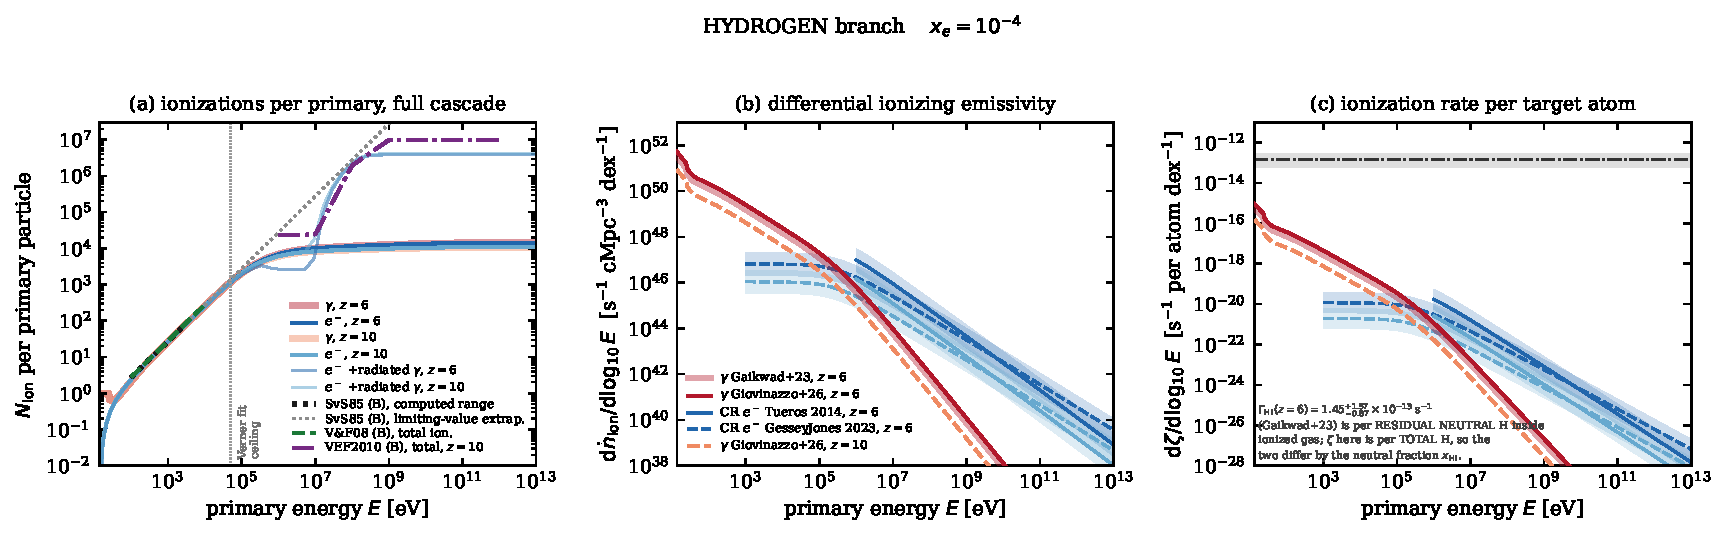
\includegraphics[width=\textwidth]{fig_ionizing_emissivity_H_xe4.pdf}
\caption{Hydrogen branch at $x_e=10^{-4}$.  (a) ionizations per primary,
engine A solid, engine B in its published ranges; (b) differential ionizing
emissivity; (c) ionization rate per target atom.  The measured
$\Gamma_{\rm H\,\textsc{i}}$ is shown for scale, with the warning that it is a
rate per \emph{residual neutral} hydrogen atom inside ionized gas whereas
$\zeta$ here is per total hydrogen, the two differing by the neutral fraction.
The equivalent figures for the other three $x_e$ values, and the eight helium
panels, are in \texttt{figures\_emissivity/}.}
\label{fig:main}
\end{figure}

\begin{figure}[htbp]
\centering
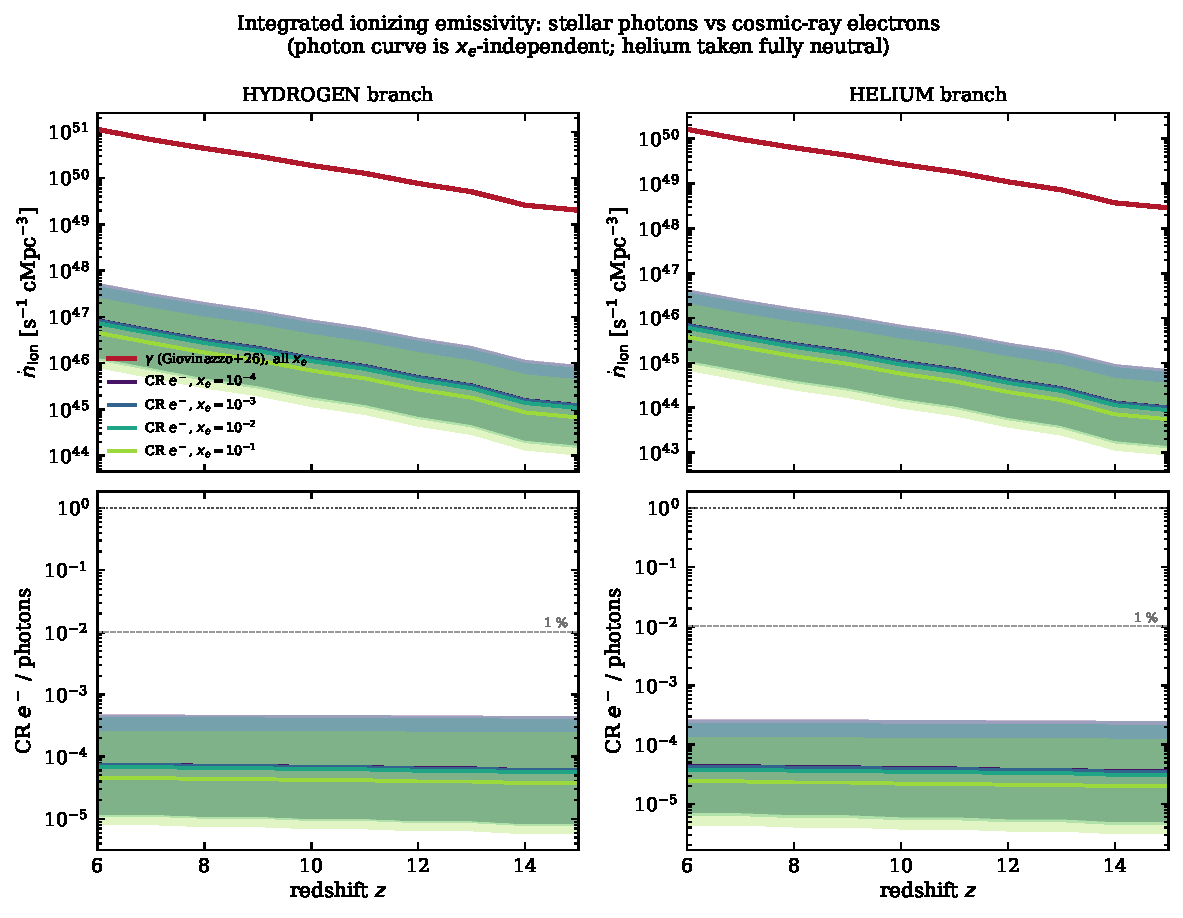
\includegraphics[width=0.92\textwidth]{fig_emissivity_vs_z.pdf}
\caption{Integrated ionizing emissivity of the two populations and their
ratio, for both branches and all four $x_e$.  The redshift range is that
tabulated by \citet{Giovinazzo2026}; nothing is extrapolated beyond it.}
\label{fig:vsz}
\end{figure}

\begin{figure}[htbp]
\centering
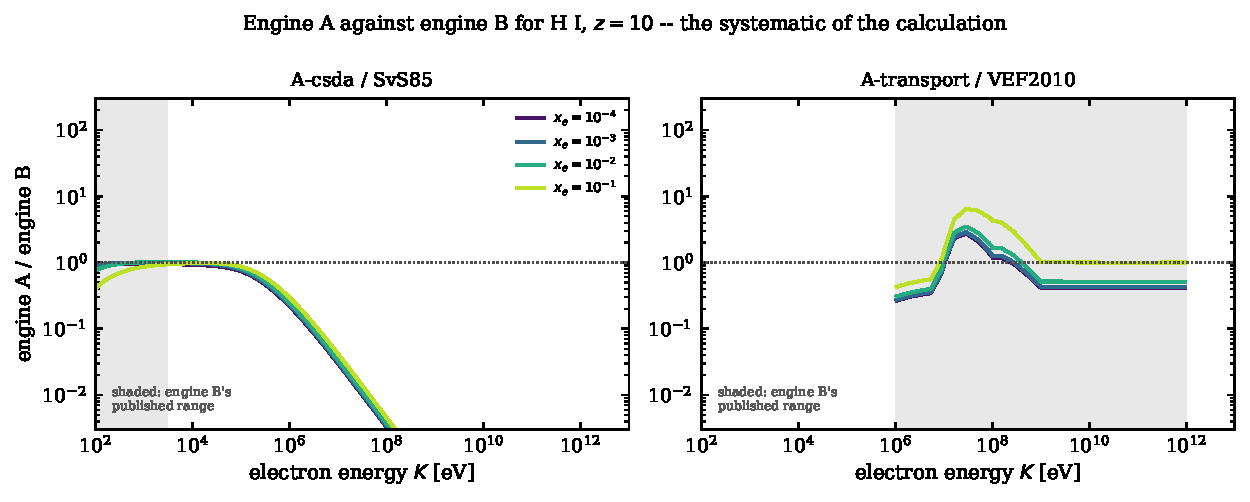
\includegraphics[width=0.92\textwidth]{fig_engine_comparison.pdf}
\caption{The systematic of the calculation: engine A against engine B over the
whole energy axis, at $z=10$, for H\,\textsc{i}.  Shaded regions mark where
engine B is inside its published range.}
\label{fig:engines}
\end{figure}

\begin{table}[htbp]
\centering
\caption{Integrated ionizing emissivity [ionizations s$^{-1}$ cMpc$^{-3}$] and
the cosmic-ray-electron share.  Photon normalisation:
\citet{Giovinazzo2026}.  The cosmic-ray range spans both injection spectra and
$\eta_{\rm cr}=0.1$--$0.5$, $f_e = 0.01$--$0.02$.}
\label{tab:final}
\begin{tabular}{ccccccc}
\toprule
& & \multicolumn{2}{c}{HYDROGEN} & \multicolumn{2}{c}{HELIUM} \\
\cmidrule(lr){3-4}\cmidrule(lr){5-6}
$z$ & $x_e$ & $\dot n_{\rm ion}^\gamma$ & CR $e^-$/$\gamma$
 & $\dot n_{\rm ion}^\gamma$ & CR $e^-$/$\gamma$ \\
\midrule
6  & $10^{-4}$ & $1.14\times10^{51}$ & $7.5\times10^{-5}$ & $1.62\times10^{50}$ & $4.4\times10^{-5}$\\
6  & $10^{-1}$ & $1.00\times10^{51}$ & $4.6\times10^{-5}$ & $1.58\times10^{50}$ & $2.4\times10^{-5}$\\
8  & $10^{-4}$ & $4.42\times10^{50}$ & $7.2\times10^{-5}$ & --- & ---\\
10 & $10^{-4}$ & $1.89\times10^{50}$ & $6.8\times10^{-5}$ & --- & ---\\
12 & $10^{-4}$ & $7.68\times10^{49}$ & $6.5\times10^{-5}$ & --- & ---\\
15 & $10^{-4}$ & $2.02\times10^{49}$ & $6.1\times10^{-5}$ & --- & ---\\
15 & $10^{-1}$ & $1.78\times10^{49}$ & $3.7\times10^{-5}$ & --- & ---\\
\bottomrule
\end{tabular}
\end{table}

\paragraph{The answer.}
\begin{equation}
  \boxed{\;
  \frac{\dot n_{\rm ion}^{{\rm CR}\,e^-}}{\dot n_{\rm ion}^{\gamma}}
  = \big(3.8\text{--}7.5\big)\times10^{-5} \ \ ({\rm H}),
  \qquad
  \big(2.0\text{--}4.4\big)\times10^{-5}\ \ ({\rm He}),
  \;}
\end{equation}
over $6\le z\le15$ and $10^{-4}\le x_e\le10^{-1}$ using the geometric mean of
the two injection prescriptions.  Including their full span and the
$\eta_{\rm cr}$, $f_e$ ranges, the hydrogen share is
$5.8\times10^{-6}$--$4.7\times10^{-4}$ and the helium share
$3.1\times10^{-6}$--$2.7\times10^{-4}$.  The ratio is remarkably flat: it
falls by only 20 per cent from $z=6$ to $z=15$ (because both populations are
tied to the same star formation history) and by a further 40 per cent from
$x_e=10^{-4}$ to $10^{-1}$ (because the cosmic-ray electrons lose an
increasing share of their energy to Coulomb heating while the photons do not).

\paragraph{What the headline ratio does and does not depend on.}
Because the cosmic-ray budget is obtained by inverting
$\dot n_{\rm ion} = f_{\rm esc}\xi_{\rm ion}\rho_{\rm SFR}$, the photon
emissivity appears in \emph{both} the numerator and the denominator of the
ratio and cancels exactly.  Swapping the \citet{Giovinazzo2026} normalisation
for the \citet{Gaikwad2023} one changes $\dot n_{\rm ion}$ by a factor
$1.601$ and changes the ratio by a factor $1.0000000000$ (verified
numerically).  \emph{The $\pm0.09$~dex uncertainty on the JWST emissivity, and
Gaikwad's asymmetric errors, therefore do not propagate into the answer at
all.}  What does propagate is
\begin{equation}
  \frac{\dot n_{\rm ion}^{{\rm CR}\,e^-}}{\dot n_{\rm ion}^{\gamma}}
  \;\propto\;
  \frac{\eta_{\rm cr}\,f_e\,E_{\rm SN}}
       {f_{\rm esc}\,\xi_{\rm ion}\,(M_\ast/N_{\rm CCSN})} ,
\end{equation}
so the escape fraction is the dominant lever: adopting
\citeauthor{Munoz2024}'s best-fit $\langle f_{\rm esc}\rangle_{\rm ion}=0.05$
instead of the \citet{Robertson2015} fiducial $0.2$ raises the ratio by a
factor 4, to $\sim1.5\times10^{-4}$ --- still four orders of magnitude below
the photon channel, but the flatness of the curves in Fig.~\ref{fig:vsz}
should not be read as insensitivity to $f_{\rm esc}$.
\flag{$f_e$, the electron share of the cosmic-ray energy, is the least
constrained link and has not been calibrated at high redshift.}

\paragraph{Where the two populations do compete.}
Panels~(b) and~(c) show the one place cosmic rays are not negligible: above
$\sim10^{6}$~eV the photon emissivity has fallen off the end of the
$E^{-\alpha_s-1}$ spectrum, while the cosmic-ray spectrum is still there.  The
crossover is at $E\simeq3$--$6\times10^{6}$~eV, and above it cosmic-ray
electrons dominate the \emph{differential} emissivity by orders of magnitude.
This is energetically irrelevant --- the integral is dominated by the decade
above 13.6~eV --- but it is the correct statement of where a cosmic-ray
signature would have to be looked for.

%=======================================================================
\section{Caveats and flagged items}\label{sec:caveats}
%=======================================================================
\begin{enumerate}\itemsep3pt
\item \flag{Helium fully neutral} at all $x_e$, by instruction.  Upper bound;
  the consistent alternative would lower the helium emissivity by
  $\le10$ per cent.
\item \flag{Engine B's helium column} inherits
  \citeauthor{ShullVanSteenberg1985}'s $n({\rm He})/n({\rm H})=0.1$ and their
  $x_{\rm He^+}=x_{\rm H^+}$, neither of which matches the assumptions used
  for engine A.  The helium engine-A/B ratio is therefore quoted only as an
  order-of-magnitude consistency check.
\item \flag{Verner et al.\ above 50~keV} is an extrapolation of a fit, using
  the correct non-relativistic asymptote.  Marked on every panel~(a).
\item \flag{No spectral index from \citet{Giovinazzo2026}}; $\alpha_s=2.0\pm0.6$
  from \citet{Gaikwad2023} is used for both photon normalisations.  Varying
  $\alpha_s$ over its $1\sigma$ range changes the H\,\textsc{i} emissivity
  integral by $\mp$ a few per cent and the He\,\textsc{i} one by more, since
  helium samples the spectrum above 24.6~eV.
\item \flag{A-transport exists only at $x_e=10^{-4}$}; the other three $x_e$
  values carry A-csda alone above 1~MeV, which omits the re-absorbed radiated
  photons and is therefore a lower bound there.
\item \flag{Three project-internal inconsistencies} surfaced by the audit and
  not repaired here, because they live in files outside this task's scope:
  \texttt{Notebooks/redo/stage9\_budget.py} uses $X=0.760$ and $m_p$ rather
  than $X_p = 1-Y_p = 0.7546$ and $m_{\rm H}$ (a $+0.99$ per cent error in
  $n_{\rm H}$); \texttt{igm\_losses.N\_HI\_NORM} $=1.8\times10^{3}\,{\rm
  m^{-3}}$ is $+2.6$ per cent above the Planck-consistent
  $1754.6\,{\rm m^{-3}}$; and \texttt{igm\_losses.THRESHOLD\_EV\_ION} uses the
  Rydberg $13.6057$~eV rather than the NIST hydrogen ionization potential
  $13.598$~eV ($+0.057$ per cent).
\item \flag{Two literature findings}, Sect.~\ref{sec:verif}G and~H, are
  reported as observations about published material, not as corrections.
\item \flag{Not covered by any pass/fail test}, and reported rather than
  asserted: the H\,\textsc{i}/He\,\textsc{i} split (engine A gives
  $f_{\rm HeI}/f_{\rm HI}\to0.0871$ against $0.0637$ from
  \citeauthor{ShullVanSteenberg1985} rescaled to the Planck helium abundance,
  a 37 per cent difference that cannot be resolved because their helium fits
  assume $x_{\rm HeII}=x_{\rm HII}$); and the two photon emissivity
  normalisations, which are inputs that nothing here can falsify.  The split
  is however shown to be insensitive to the shape of $\Lambda$: tripling the
  helium term moves $f_{\rm HeI}$ by 2.8 per cent at 100~eV and $<0.2$ per
  cent above 1~keV, which is the derivation's own claim.
\item \flag{Provenance of the anchors.}  Neither photon normalisation is a raw
  measurement: \citet{Gaikwad2023} calibrate against simulations of the
  Ly$\alpha$ forest, and \citet{Giovinazzo2026} infer $\dot n_{\rm ion}$ from
  SED fitting with an assumed escape prescription.
\end{enumerate}

%=======================================================================
\section*{Reproducibility}
%=======================================================================
All code in \texttt{State of the art - Reionization/ionizing\_emissivity/}.
No stochastic method is used anywhere, so no random seed is involved.
\begin{itemize}\itemsep1pt
\item \texttt{emis\_common.py} --- constants, cosmology, Verner cross-sections.
\item \texttt{emis\_engine\_A.py} and \texttt{emis\_engine\_A\_xe.py} ---
  engine A and its extended CSDA cache,\\
  \texttt{emis\_engineA\_cache\_ext.npz}.
\item \texttt{emis\_engine\_B.py} --- SvS85, V\&F08 and the parser for the
  VEF2010 appendix tables.
\item \texttt{emis\_sources.py} --- the four normalisations and the IMF integral.
\item \texttt{emis\_figure.py} and \texttt{emis\_summary\_figure.py} $\to$\\
  \texttt{figures\_emissivity/} (8 branch figures + 2 summary figures).
\item \texttt{emis\_verify.py} $\to$ \texttt{emis\_verify.log};\\
  \texttt{emis\_results.txt} holds the tabulated results.
\item Papers added to \texttt{Agents/}: \citet{Verner1996},
  \citet{ShullVanSteenberg1985}, \citet{ValdesFerrara2008},
  \citet{Valdes2010}.
\end{itemize}

\begin{thebibliography}{99}
\bibitem[Berezinskii et al.(1990)]{Berezinskii1990} Berezinskii, V.~S., et al. 1990, Astrophysics of Cosmic Rays (Amsterdam: North-Holland).
\bibitem[Blumenthal \& Gould(1970)]{BlumenthalGould1970} Blumenthal, G.~R., \& Gould, R.~J. 1970, Rev.\ Mod.\ Phys., 42, 237.
\bibitem[Caprioli \& Spitkovsky(2014)]{CaprioliSpitkovsky2014} Caprioli, D., \& Spitkovsky, A. 2014, ApJ, 783, 91.
\bibitem[Chabrier(2003)]{Chabrier2003} Chabrier, G. 2003, PASP, 115, 763.
\bibitem[Drury(1983)]{Drury1983} Drury, L.~O'C. 1983, Rep.\ Prog.\ Phys., 46, 973.
\bibitem[Drury et al.(1989)]{Drury1989} Drury, L.~O'C., Markiewicz, W.~J., \& V\"olk, H.~J. 1989, A\&A, 225, 179.
\bibitem[Fixsen(2009)]{Fixsen2009} Fixsen, D.~J. 2009, ApJ, 707, 916.
\bibitem[Gaikwad et al.(2023)]{Gaikwad2023} Gaikwad, P., et al. 2023, MNRAS, 525, 4093 (arXiv:2304.02038).
\bibitem[Gessey-Jones et al.(2023)]{GesseyJones2023} Gessey-Jones, T., et al. 2023, MNRAS, 526, 4262 (arXiv:2304.07201).
\bibitem[Giovinazzo et al.(2026)]{Giovinazzo2026} Giovinazzo, E., et al. 2026, arXiv:2607.22834.
\bibitem[Gould(1972)]{Gould1972} Gould, R.~J. 1972, Physica, 60, 145.
\bibitem[Kim \& Rudd(1994)]{KimRudd1994} Kim, Y.-K., \& Rudd, M.~E. 1994, Phys.\ Rev.\ A, 50, 3954.
\bibitem[Kim et al.(2000)]{Kim2000} Kim, Y.-K., Santos, J.~P., \& Parente, F. 2000, Phys.\ Rev.\ A, 62, 052710.
\bibitem[Mu\~noz et al.(2024)]{Munoz2024} Mu\~noz, J.~B., Mirocha, J., Chisholm, J., Furlanetto, S.~R., \& Mason, C. 2024, MNRAS, 535, L37 (arXiv:2404.07250).
\bibitem[Planck Collaboration(2020)]{Planck2018} Planck Collaboration 2020, A\&A, 641, A6 (arXiv:1807.06209).
\bibitem[Robertson et al.(2015)]{Robertson2015} Robertson, B.~E., et al. 2015, ApJ, 802, L19 (arXiv:1502.02024).
\bibitem[Shull \& van Steenberg(1985)]{ShullVanSteenberg1985} Shull, J.~M., \& van Steenberg, M.~E. 1985, ApJ, 298, 268.
\bibitem[Stone \& Kim(2002)]{StoneKim2002} Stone, P.~M., \& Kim, Y.-K. 2002, J.\ Phys.\ B, 35, 1675.
\bibitem[Tueros et al.(2014)]{Tueros2014} Tueros, M., del Valle, M.~V., \& Romero, G.~E. 2014, A\&A, 570, L4 (arXiv:1409.6225).
\bibitem[Vald\'es \& Ferrara(2008)]{ValdesFerrara2008} Vald\'es, M., \& Ferrara, A. 2008, MNRAS, 387, L8 (arXiv:0803.0370).
\bibitem[Vald\'es et al.(2010)]{Valdes2010} Vald\'es, M., Evoli, C., \& Ferrara, A. 2010, MNRAS, 404, 1569 (arXiv:0911.1125).
\bibitem[Verner et al.(1996)]{Verner1996} Verner, D.~A., Ferland, G.~J., Korista, K.~T., \& Yakovlev, D.~G. 1996, ApJ, 465, 487 (arXiv:astro-ph/9601009).
\bibitem[Woosley \& Weaver(1995)]{WoosleyWeaver1995} Woosley, S.~E., \& Weaver, T.~A. 1995, ApJS, 101, 181.
\end{thebibliography}

\end{document}
